\documentclass[
	12pt,				% tamanho da fonte
	openright,			% capítulos começam em pág ímpar (insere página vazia caso preciso)
	twoside,			% twoside para impressão em verso e anverso. Oposto a oneside
	a4paper,			% tamanho do papel. 
	% -- opções do pacote babel --
	english,			% idioma adicional para hifenização
	french,				% idioma adicional para hifenização
	spanish,			% idioma adicional para hifenização
	brazil				% o último idioma é o principal do documento
	]{abntex2}

% ---
% Pacotes básicos 
% ---

\usepackage[utf8]{inputenc}
\usepackage{graphicx}
\usepackage[section]{placeins}
\usepackage{setspace}
\usepackage{fontenc}
\usepackage{listings}
\usepackage{color}
\usepackage{url}
\usepackage[printonlyused]{acronym}
\usepackage{rotating}
\usepackage{bytefield}
\usepackage[table]{xcolor}
\usepackage{multirow}
\usepackage{subfigure}
\usepackage{lscape}
\usepackage{enumitem}
\usepackage{fixltx2e}
\usepackage{longtable}
\usepackage{mathtools}
\usepackage{tabularx}
\usepackage{adjustbox}
\usepackage{amsmath}
\usepackage{booktabs}
\usepackage{textcomp} 
\usepackage{array}
\usepackage{booktabs}
\usepackage{xcolor}
\usepackage{colortbl}



\usepackage{adjustbox}
\usepackage{amsmath}
\usepackage[printonlyused]{acronym}
\usepackage{lmodern}			% Usa a fonte Latin Modern			
%\usepackage{uarial}
%\renewcommand{\familydefault}{\sfdefault}
\usepackage[T1]{fontenc}		% Selecao de codigos de fonte.
\usepackage[utf8]{inputenc}		% Codificacao do documento (conversão automática dos acentos)
\usepackage{lastpage}			% Usado pela Ficha catalográfica
\usepackage{indentfirst}		% Indenta o primeiro parágrafo de cada seção.
\usepackage{color}				% Controle das cores
\usepackage{graphicx}			% Inclusão de gráficos
\usepackage{microtype} 			% para melhorias de justificação
\usepackage[brazilian,hyperpageref]{backref}	 % Paginas com as citações na bibl
\usepackage[alf]{abntex2cite}	% Citações padrão ABNT
\usepackage[table]{xcolor}
\usepackage{multirow}
% --- 
% CONFIGURAÇÕES DE PACOTES
% --- 

% ---
% Configurações do pacote backref
% Usado sem a opção hyperpageref de backref
\renewcommand{\backrefpagesname}{Citado na(s) página(s):~}
% Texto padrão antes do número das páginas
\renewcommand{\backref}{}
% Define os textos da citação
\renewcommand*{\backrefalt}[4]{
	\ifcase #1 %
		Nenhuma citação no texto.%
	\or
		Citado na página #2.%
	\else
		Citado #1 vezes nas páginas #2.%
	\fi}%
% ---

% ---
% Informações de dados para CAPA e FOLHA DE ROSTO
% ---
\titulo{O Uso de Processamento de Linguagem Natural para a Análise de
Sentimentos na Rede Social Reddit}
\autor{Guilherme Henrique Santos Andreata}
\local{Caxias do Sul}
\data{2017}
\orientador{André Luis Martinotto}
\instituicao{%
UNIVERSIDADE DE CAXIAS DO SUL
\par
CENTRO DE COMPUTAÇÃO E TECNOLOGIA DA INFORMAÇÃO
\par
BACHARELADO EM SISTEMAS DE INFORMAÇÃO}
\tipotrabalho{Projeto de Diplomação}
% O preambulo deve conter o tipo do trabalho, o objetivo, 
% o nome da instituição e a área de concentração 
\preambulo{Projeto de Diplomação submetido ao curso de Bacharelado em
Sistemas de Informação do Centro de Computação e Tecnologia da
Informação da Universidade de Caxias do Sul, como requisito obrigatório para graduação.}
% ---

% alterando o aspecto da cor azul
\definecolor{blue}{RGB}{2,2,2}

% informações do PDF
\makeatletter
\hypersetup{
     	%pagebackref=true,
		pdftitle={\@title}, 
		pdfauthor={\@author},
    	pdfsubject={\imprimirpreambulo},
	    pdfcreator={LaTeX with abnTeX2},
		pdfkeywords={abnt}{latex}{abntex}{abntex2}{trabalho acadêmico}, 
		colorlinks=true,       		% false: boxed links; true: colored links
    	linkcolor=blue,          	% color of internal links
    	citecolor=blue,        		% color of links to bibliography
    	filecolor=magenta,      		% color of file links
		urlcolor=blue,
		bookmarksdepth=4
}
\makeatother 
% --- 

% --- 
% Espaçamentos entre linhas e parágrafos 
% --- 

% O tamanho do parágrafo é dado por:
\setlength{\parindent}{1.3cm}

% Controle do espaçamento entre um parágrafo e outro:
\setlength{\parskip}{0.2cm}  % tente também \onelineskip

% ---
% compila o indice
% ---
\makeindex
% ---

% ----
% Início do documento
% ----
\begin{document}

% Retira espaço extra obsoleto entre as frases.
\frenchspacing 

% ----------------------------------------------------------
% ELEMENTOS PRÉ-TEXTUAIS
% ----------------------------------------------------------
% \pretextual

% ---
% Capa
% ---
\imprimircapa
% ---

% ---
% Folha de rosto
% (o * indica que haverá a ficha bibliográfica)
% ---
\imprimirfolhaderosto*
% ---

% ---
% Inserir a ficha bibliografica
% ---
%
% Isto é um exemplo de Ficha Catalográfica, ou ``Dados internacionais de
% catalogação-na-publicação''. Você pode utilizar este modelo como referência. 
% Porém, provavelmente a biblioteca da sua universidade lhe fornecerá um PDF
% com a ficha catalográfica definitiva após a defesa do trabalho. Quando estiver
% com o documento, salve-o como PDF no diretório do seu projeto e substitua todo
% o conteúdo de implementação deste arquivo pelo comando abaixo:
%
% \begin{fichacatalografica}
%     \includepdf{fig_ficha_catalografica.pdf}
% \end{fichacatalografica}
\begin{fichacatalografica}
	\vspace*{\fill}					% Posição vertical
	\hrule							% Linha horizontal
	\begin{center}					% Minipage Centralizado
	\begin{minipage}[c]{12.5cm}		% Largura
	
	\imprimirautor
	
	\hspace{0.5cm} \imprimirtitulo  / \imprimirautor. --
	\imprimirlocal, \imprimirdata-
	
	\hspace{0.5cm} \pageref{LastPage} p. : il. (algumas color.), 30 cm.\\
	
	\hspace{0.5cm} \imprimirorientadorRotulo~\imprimirorientador\\
	
	\hspace{0.5cm}
	\parbox[t]{\textwidth}{\imprimirtipotrabalho~--~\imprimirinstituicao,
	\imprimirdata.}\\
	
	\hspace{0.5cm}
		1. AMQP.
		2. \textit{Analytic Hierarchy Process}.
		I. André Luis Martinotto.
		II. Universidade de Caxias do Sul.
		III. Faculdade de Ciências da Computação.
		IV. Avaliação de intermediadores de mensagem que implementam o protocolo \textit{AMQP}\\ 			
	
	\hspace{8.75cm} CDU 02:141:005.7\\
	
	\end{minipage}
	\end{center}
	\hrule
\end{fichacatalografica}
% ---

% ---
% Inserir folha de aprovação
% ---
\cleardoublepage
% Isto é um exemplo de Folha de aprovação, elemento obrigatório da NBR
% 14724/2011 (seção 4.2.1.3). Você pode utilizar este modelo até a aprovação
% do trabalho. Após isso, substitua todo o conteúdo deste arquivo por uma
% imagem da página assinada pela banca com o comando abaixo:
%
% \includepdf{folhadeaprovacao_final.pdf}
%
\begin{folhadeaprovacao}

  \begin{center}
    {\ABNTEXchapterfont\large\imprimirautor}

    \vspace*{\fill}\vspace*{\fill}
    \begin{center}
      \ABNTEXchapterfont\bfseries\Large\imprimirtitulo
    \end{center}
    \vspace*{\fill}
    
    \hspace{.45\textwidth}
    \begin{minipage}{.5\textwidth}
        \imprimirpreambulo
    \end{minipage}%
    \vspace*{\fill}
   \end{center}
        
   %\imprimirlocal, 02 de dezembro de 2015: 

   \assinatura{\textbf{\imprimirorientador} \\ Orientador} 
   \assinatura{\textbf{Daniel Luís Notari} \\ Convidado 1}
   \assinatura{\textbf{Helena Graziottin Ribeiro} \\ Convidado 2}
   %\assinatura{\textbf{Professor} \\ Convidado 3}
   %\assinatura{\textbf{Professor} \\ Convidado 4}
      
   \begin{center}
    \vspace*{0.5cm}
    {\large\imprimirlocal}
    \par
    {\large\imprimirdata}
    \vspace*{1cm}
  \end{center}
  
\end{folhadeaprovacao}
% ---

% ---
% Dedicatória
% ---
%\begin{dedicatoria}
   \vspace*{\fill}
   \centering
   \noindent
   \textit{ Este trabalho é dedicado às crianças adultas que,\\
   quando pequenas, sonharam em se tornar cientistas.} \vspace*{\fill}
\end{dedicatoria} 
% ---

% ---
% Agradecimentos
% ---
%\begin{agradecimentos}
Os agradecimentos principais são direcionados à Gerald Weber, Miguel Frasson,
Leslie H. Watter, Bruno Parente Lima, Flávio de Vasconcellos Corrêa, Otavio Real
Salvador, Renato Machnievscz\footnote{Os nomes dos integrantes do primeiro
projeto abn\TeX\ foram extraídos de
\url{http://codigolivre.org.br/projects/abntex/}} e todos aqueles que
contribuíram para que a produção de trabalhos acadêmicos conforme
as normas ABNT com \LaTeX\ fosse possível.

Agradecimentos especiais são direcionados ao Centro de Pesquisa em Arquitetura
da Informação\footnote{\url{http://www.cpai.unb.br/}} da Universidade de
Brasília (CPAI), ao grupo de usuários
\emph{latex-br}\footnote{\url{http://groups.google.com/group/latex-br}} e aos
novos voluntários do grupo
\emph{\abnTeX}\footnote{\url{http://groups.google.com/group/abntex2} e
\url{http://abntex2.googlecode.com/}}~que contribuíram e que ainda
contribuirão para a evolução do \abnTeX.

\end{agradecimentos}
% ---

% ---
% RESUMOS
% ---
% resumo em português
\setlength{\absparsep}{18pt} % ajusta o espaçamento dos parágrafos do resumo
\begin{resumo}
A sociedade tem cada vez mais expressado a sua opinião através de Redes
Sociais, sendo que entre essas se destaca o
Reddit. De fato, essa é uma das maiores redes sociais no mundo, com mais de 17
milhões de usuários. Nesta, os usuários podem postar \textit{links}, bem como
comentários sobre estes, gerando um grande volume de dados que muitas vezes são
ignorados.

A identificação de padrões de sentimentos expressos por grupos dessa comunidade,
se torna útil visto que a partir dessa avaliação é possível construir
ferramentas que podem apoiar decisões do ponto de vista político, econômico, etc. Por exemplo, a partir desta análise, é
possível identificar a opinião dos usuários em relação a um candidato em uma eleição ou ainda a aceitação dos
consumidores em relação a um novo produto.

Assim, neste trabalho foi desenvolvido um \textit{software} que permite efetuar
a análise de sentimentos na rede social Reddit. Esse foi desenvolvido
utilizando o método de \ac{VADER}, que se encontra implementado no
\textit{framework} \ac{NLTK}.

Além disso, utilizou-se o Método de Propagação Dupla, com a escolha de palavras
alvos. A partir dessa implementação obteve-se uma assertividade de 59,17\% na
avaliação de comentários de política e 72,54\% na avaliação de comentários sobre
filmes.


 \textbf{Palavras-chaves}: Reddit. Processamento de Linguagem Natural. Análise de Sentimentos.
\end{resumo}

% resumo em inglês
\begin{resumo}[Abstract]
 \begin{otherlanguage*}{english}
   The society has been increasingly expressing themselves through social networks,
which from among those, the one who stand out is Reddit. Indeed, this is one of
the biggest social networks in the world with more than 17 millions of users. At
this, users can send links, as well as comment on these, generating a big volume
of data, which a lot of times get ignored.

The recognition of sentiment patterns expressed by groups of that community
make itself useful because from that evaluation, is possible the build tools
that can support decisions from an economic point of views, political
point of view, etc. For an example, with that
analysis, it is possible to identify the users's opinion regarding an election candidate or the costumers's acceptance of a new product.

Therefore, in this work was developed a software capable of performing a
sentiment analysis on the Reddit social network. This was developed using
the \ac{VADER} method which is implemented by the \ac{NLTK} \textit{framework}.

Furthermore, it was utilized the Double Propagation Method with the choosing of
a target word. From that implementation we got a 59,17\% accuracy evaluating
political commentaries and 72,54\% accuracy evaluating movie reviews
commentaries. 

   \vspace{\onelineskip}
 
   \noindent 
   \textbf{Key-words}: Reddit. Natural Language Processing. Sentiment
Analysis.
 \end{otherlanguage*}
\end{resumo}
% ---

% ---
% inserir lista de ilustrações
% ---


\pdfbookmark[0]{\listfigurename}{lof}
\listoffigures*
\cleardoublepage
% ---

% ---
% inserir lista de tabelas
% ---
\pdfbookmark[0]{\listtablename}{lot}
\listoftables*
\cleardoublepage
% ---

% ---
% inserir lista de abreviaturas e siglas
% ---
\chapter*{Lista de acrônimos}

\vspace{20px}
\begin{acronym}[XXXXXXXXXX]
\acro{NLP}[NLP]{\textit{Natural Language Processing}}
\acro{NLTK}[NLTK]{\textit{Natural Language Toolkit}}
\acro{MaxEnt}[MaxEnt]{\textit{Maximum Entropy}}
\acro{RNTN}[RNTN]{\textit{Recursive Neural Tensor Networks}}
\acro{VADER}[VADER]{\textit{Valence Aware Dictionary and sEntiment Reasoner}}
\acro{JSON}[JSON]{\textit{JavaScript Object Notation}}
\acro{POJO}[POJO]{\textit{Plain Old Java Objects}}
\acro{SVM}[SVM]{\textit{Support Vector Machines}}
\acro{API}[API]{\textit{Application Programming Interface}}
\end{acronym}

\cleardoublepage
% ---
% inserir o sumario
% ---
\pdfbookmark[0]{\contentsname}{toc}
\tableofcontents*
\cleardoublepage
% ---

% ----------------------------------------------------------
% ELEMENTOS TEXTUAIS
% ----------------------------------------------------------
\textual
\chapter{Introdução}
\label{chap:introducao}
A linguagem é a forma com que nós nos comunicamos, seja ela escrita ou
falada, através de símbolos ou sons. De fato, a linguagem é a forma como
expressamos nossas idéias, sentimentos e experiências. O Processamento de
Linguagem Natural, é o termo utilizado para descrever um software ou componente
de hardware que tem como função analisar a linguagem escrita ou falada
\cite{jacksonmoulinier2007}.

Existem duas abordagens de Processamento de Linguagem Natural, sendo a primeira
delas é chamada de simbólica ou racionalista e a outra de empírica. A primeira
abordagem consiste em uma série de regras para a manipulação de símbolos, como as regras gramaticais que permitem identificar se uma frase está malformada ou não. A abordagem
empírica está centrada na análise estatística da linguagem através de grandes quantidades
de textos, como por exemplo, a utilização de modelos de Markov para reconhecer padrões
na escrita \cite{jacksonmoulinier2007}.

Existem diversos \textit{frameworks open source} que facilitam o desenvolvimento
de \textit{software} para o Processamento de Linguagem Natural, sendo que entre
esses destacam-se o \textit{Stanford's Core NLP Suite} \cite{corenlp}, \textit{Natural Language
Toolkit} \cite{nltk}, \textit{Apache OpenNLP} \cite{opennlp} e \textit{Spacy}
\cite{spacy}.
Esses \textit{frameworks} nos permitem, entre outras coisas, efetuar análise de
sentimentos, identificar tópicos e conteúdos.

A rede social Reddit é o vigésimo terceiro \textit{website} mais acessado na
internet e o sétimo mais acessado nos Estados Unidos da América \cite{alexa}.
Através deste \textit{website}, seus usuários podem criar ou se inscrever em
comunidades, também conhecidas como \textit{subreddits}.
Uma vez que as comunidades são criadas pelos próprios usuários, podemos encontrar
comunidades sobre todos os assuntos, sejam notícias do mundo, comunidades
partidárias, comunidades criadas para pessoas de uma mesma localidade ou comunidades
de imagens engraçadas.

Nestas comunidades é possível visualizar e comentar \textit{links} enviados por
outros usuários.
Além disso, o usuário pode efetuar um voto de forma positiva, caso acredite que
aquele \textit{link} é útil para a comunidade. Caso contrário, é possível
efetuar um voto negativo.
Uma vez que os próprios usuários podem submeter \textit{links}, os eventos e
notícias de todo o mundo são reportados no \textit{website}, como exemplo,
pode-se citar as eleições ocorridas no ano de 2016 nos Estados Unidos e o
tiroteio ocorrido em Paris.

Neste trabalho será desenvolvido um software que permita realizar a
análise dos comentários do \textit{website} Reddit. Mais
especificamente esses comentários serão analisados com o objetivo de identificar padrões de sentimentos, ou seja, determinar se a
opinião expressada com relação a um determinado tópico é neutra, positiva ou negativa.

\section{Objetivos do Trabalho}

Este trabalho tem como objetivo a análise dos comentários disponíveis no
\textit{website} Reddit, identificando padrões de sentimentos entre os
usuários de suas comunidades. De forma a atingir o objetivo principal desse
trabalho, os seguintes objetivos específicos devem ser realizados:
\begin{itemize}
  \item Desenvolver uma ferramenta para o Processamento Natural de Linguagem através de
\textit{frameworks} já existentes.
 \item Construção de uma base de dados a partir do \textit{website} Reddit.
 \item Efetuar o processamento da base de dados utilizando a ferramenta desenvolvida.
\end{itemize}

\section{Estrutura do Trabalho}
%O presente trabalho está estruturado da seguinte forma: no Capítulo
% \ref{cap:Animacao} será apresentada a história da animação, seu surgimento e conceitos. No Capítulo \ref{cap:Blender} são apresentadas informações sobre o \textit{software} Blender, assim como os métodos disponíveis nesse para a criação de animações 3D. No Capítulo \ref{cap:Kinect} será apresentado o sensor Kinect, assim como seu funcionamento e alguns conceitos sobre as imagens capturadas. No Capítulo \ref{cap:DesenvKinect} serão apresentadas as bibliotecas e ferramentas para o desenvolvimento de aplicações utilizando Kinect. Além disso, é realizado um comparativo, onde são apresentadas as vantagens e desvantagens de cada uma dessas ferramentas. No Capítulo \ref{cap:AplicaIntegra} serão apresentados alguns \textit{softwares} que já fazem a integração entre o sensor e a ferramenta, assim como o funcionamento desses. No Capítulo \ref{cap:Implementacao} serão apresentados os detalhes da solução desenvolvida e da animação gerada, bem como são apresentados os testes realizados e os resultados obtidos. Por fim, no Capítulo \ref{cap:Consideracoes} são apresentadas as considerações finais e sugestões de trabalhos futuros.

\chapter{Processamento de Linguagem Natural}
\label{cap:Processamento}

% Um computador, obviamente, está preparado para entender sua própria linguagem,
% como por exemplo, um compilador interpreta linhas de código fonte para gerar um
% programa executável seguindo exatamente o algoritmo utilizado. Por isso, temos o
% termo Natural no Processamento de Linguagem. 

O objetivo da área de Processamento de Linguagem Natural é analisar a linguagem natural, ou seja, a linguagem utilizada pelo seres humanos não
importando se essa é escrita ou falada \cite{manningschutze1999}.

O Processamento de Linguagem Natural é uma área antiga, sendo anterior a
invenção dos computadores modernos. De fato, sua primeira grande aplicação foi
um dicionário desenvolvido no Birkbeck College em Londres no ano de 1948. Por ser
uma área complexa, seus primeiros trabalhos foram notavelmente falhos o que
causou uma certa hostilidade por parte das agências formentadoras de pesquisas.

Os primeiros pesquisadores eram muitas vezes bilíngues, como por exemplo,
nativos alemães que imigraram para os Estados Unidos. Acreditava-se que pelo
fato desses terem conhecimento de ambas as linguas, Ingles e Alemão, eles teriam
capacidade de desenvolver programas de computadores que efetuariam a tradução das linguas
de modo satisfatório. Uma vez que esses encontraram muitas dificuldades,
ficou claro que o maior problema não era o conhecimento de ambas as
línguas e sim como expressar esse conhecimento na forma de um programa de
computador \cite{history}.

Para que um computador seja capaz de interpretar uma
língua, necessitamos antes entender como nós efetuamos essa
interpretação.
Por isso, uma parte considerável do Processamento de Linguagem Natural está apoiado na área de Linguística.

\section{Linguística}

O objetivo da Linguística é compreender como os humanos adquirem, produzem e
entendem as diversas línguas, ou seja, a forma com que conversamos, a nossa
escrita e outras mídias de comunicação \cite{manningschutze1999}.

Na linguagem tanto escrita, como na falada, existem regras que são utilizadas
para estruturar as expressões. Uma série de dificuldades no Processamento de
Linguagem Natural são ocasionadas pelo fato de que as pessoas constantemente
mudam essas regras para satisfazerem suas necessidades de comunicação
\cite{manningschutze1999}. Uma vez que as regras são constantemente modificadas pelo loucutor, se torna extremamente difícil a criação de um software ou hardware efetue a interpretação de uma língua. 


% \subsection{Sintaxe e Semântica}
% 
% No seu livro Estruturas Sintáticas, Noam Chomsky cita as seguintes frases
% ``Ideias verdes incolores dormem furiosamente'' e ``Incolores verde ideias dormem
% furiosamente''.
% 
% A primeira frase, do ponto de vista sintático é correta, porém, assim como a
% segunda frase, semânticamente não faz sentido.
% 
% O fato de que podemos modificar as regras da lingua de duas formas distintas é
% utilizado como evidência para a separação da sintaxe e semântica na língua.
% \cite{jacksonmoulinier2007}

\section{Métodos de Processamento de Linguagem Natural}

O \ac{NLP} tem como o objetivo a execução de diversas tarefas como categorização
de documentos, tradução e geração de textos a partir de um banco de dados de
computador, etc. Podemos destacar duas formas ou métodos para a execução dessas
tarefas, o método simbólico e o método estatístico, com origem o campo da linguística. 

Nos final dos anos 50 e 60, existiam excelentes métodos quantitativos
desenvolvidos durante a segunda guerra mundial para a solução de problemas
científicos \cite{shannon48}.
Porém, no ano de 1957, Chomsky publicou o seu trabalho ``Syntactic Structures''
e com isso, temos a primeira aparição da teoria de gramática gerativa, que
considera a gramática como um conjunto de regras. Essa abordagem através de um
conjunto de regras ao invés de um modelo matemático entra em conflito com os
trabalhos anteriores, criando duas comunidades no campo de Linguística. Como
reflexo das duas comunidades, a área de \ac{NLP} que crescia em paralelo a
linguística também foi dividida em duas, uma área que fazia uso de métodos que
utilizavam regras(simbólico) e uma outra área que fazia uso de métodos
quantitativos(estatísticos).


Essa seção tem como objetivo explicar os dois métodos principais de
abordagem e demonstrar as diferenças entre os dois métodos através de um exemplo
de desambiguação de categoria de palavras.


\subsection{Método Simbólico} 
O método simbólico ou racionalista está
baseado no campo da Linguística e faz o uso da manipulação dos símbolos,
significados e das regras de um texto. Um exemplo de método simbólico é o
método de Brill \cite{Brill:1992:SRP:974499.974526}. Por exemplo, no método de
Brill a frase ``João pintou a casa de branco'', será separada em palavras que
serão classificadas através de um dicionário pré-definido, como:

\begin{table}[htb]
\centering
\begin{tabular}{l|l|l|l|l|l|l}
Palavra         & João        & pintou & a      & casa        & de        
& branco
         \\
%Correta: & Substantivo & Verbo  & Artigo & Substantivo & Preposição &
% Substantivo \\
Classificação:   & 			   & Verbo  & Artigo & Substantivo & Preposição & Adjetivo
\end{tabular}
\label{my-label}
\end{table}

Observa-se que algumas palavras não foram
identificadas, como ``João'' ou classificadas de forma errada, como
``branco". Desta forma, o método utiliza-se de outras duas regras para uma
classificação inicial.
A primeira regra classifica todas as palavras desconhecidas que iniciam em
maiúsculo como substantivos, por exemplo, a palavra ``João''. Já a segunda regra, atribui para a palavra desconhecida a mesma classificação
de outras palavras que terminam com as mesmas três letras. Por exemplo, supondo
que a palavra ``pintou'' não fosse encontrada no dicionário, essa seria
associada a outras palavras terminadas com o sufixo ``tou''. Ou seja, essa seria
associada como verbo.

\begin{table}[htb]
\centering
\begin{tabular}{l|l|l|l|l|l|l}
Palavra         & João        & pintou & a      & casa        & de        
& branco
         \\
%Correta: & Substantivo & Verbo  & Artigo & Substantivo & Preposição &
% Substantivo \\
Classificação:   & \textbf{Substantivo} & Verbo  & Artigo & Substantivo &
Preposição & Adjetivo
\end{tabular}
\label{my-label}
\end{table}



Após essa classificação inicial, o método executa o seguinte conjunto de regras:

\begin{itemize}
   \item Se uma palavra tem a classificação \textbf{A} e está no contexto
  \textbf{C} então a sua classificação deverá ser mudada para \textbf{B}. Por
  exemplo, se uma palavra \textbf{A} (branco no exemplo) é um adjetivo e uma das
  duas palavras anteriores é uma preposição (``de'' no contexto \textbf{C}
  ), mude para sua classificação para substantivo (classificação \textbf{B}).
  
  \[\overbrace{\text{João}}^\text{Substantivo}
  \overbrace{\text{pintou}}^\text{Verbo}
  \overbrace{\text{a}}^\text{Artigo}
  \underbrace{
  \overbrace{\text{casa}}^\text{Substantivo}
  \overbrace{\text{de}}^\text{Preposição}}_\text{Contexto \textbf{C}}
  \underbrace{\overbrace{\text{branco}}^{\textcolor{red}{Adjetivo}}}_\text{Classificação
  \textbf{A}\textrightarrow\textbf{B}}
 \]
 
  \item Se uma palavra tem a classificação \textbf{A} e tem uma propriedade
  \textbf{P} então a sua classificação deverá ser alterada para \textbf{B}. Por
  exemplo, se uma palavra \textbf{A} (``Linda'') foi classificada como um
  adjetivo e é iniciada com uma letra maiúscula (propriedade \textbf{P}), sua
  classificação deverá ser alterada para substantivo (classificação \textbf{B}).
  
  \[\overbrace{\text{Comprei}}^\text{Verbo}
  \overbrace{\text{flores}}^\text{Substantivo}
  \overbrace{\text{para}}^\text{Preposição}
  \underbrace{\overbrace{\text{L}\text{inda}}^{\textcolor{red}{Adjetivo}}}_\text{Classificação
  \textbf{A}\textrightarrow\textbf{B}}
 \]
 
  \item Se uma palavra tem a classificação \textbf{A} e uma palavra com a
  propriedade \textbf{P} está na região \textbf{R}, sua classificação deverá
  ser \textbf{B}. Por exemplo, se uma das duas palavras anteriores (``João
  adora" na região \textbf{R}) iniciam com letra maiúscula (propriedade
  \textbf{P}), sua classificação deverá ser alterada para substantivo (classificação \textbf{B}).
  
   \[\underbrace{\overbrace{\text{João}}^\text{Substantivo}
  \overbrace{\text{adora}}^\text{Verbo}}_\text{Região \textbf{R}}
  \underbrace{\overbrace{\text{L}\text{inda}}^{\textcolor{red}{Adjetivo}}}_\text{Classificação
  \textbf{A}\textrightarrow\textbf{B}}
 \]
 
  
\end{itemize}

\subsection{Método Estatístico} 
O método estatístico ou empírico utiliza-se de grandes
quantidades de texto, procurando por padrões e
associações a modelos, sendo que esses podem ou não estarem relacionados com
regras sintáticas ou semânticas. Como exemplo, podemos citar a utilização de
Modelos de Markov pela algoritmo de Viterbi. Onde, a partir de um conjunto de
dados já classificados, ou seja, um \textit{training set} é verificada a
possibilidade de transição entre as classes gramaticais.
Por exemplo, se no nosso \textit{training set}, temos 10000 substantivos que em
7000 dos casos são seguidos por um verbo, temos:

\[ P(VB|SM) = \frac{C(SM,VB)}{C(SM)} = \frac{7000}{10000} = 0.7 \]

Onde \textbf{VB} são verbos e \textbf{SM} substantivos. Como pode ser observado
na equação, a probabilidade de um substantivo ser seguido de um verbo
(\textbf{(VB$\vert$SM)}) é igual a ocorrência de substantivos seguidos de verbos (\textbf{C(SM,VB)})
dividida pela quantidade total de substantivos em nosso \textit{training set}.

Após, é calculada a probabilidade de cada palavra ser associada com uma classe.
Supondo que dos 10000 substantivos, 150 são a palavra ``um'' classificada
dentre artigo, substantivo e pronome, como substantivo:

\[ P(um|SM) = \frac{C(SM,um)}{C(SM)} = \frac{150}{10000} = 0.015 \]

Aonde que \textbf{um} é a palavra que está sendo classificada e \textbf{SM}
são os substantivos existentes no nosso \textit{training set}. Portanto a
probabilidade de um substantivo ser associada a palavra ``um''
(\textbf{P(um$\vert$SM)}) é igual a quantidade da palavra ``um''
classificada como substantivo (\textbf{C(SM,um)}) dividida pela quantidade de
substantivos em nosso \textit{training set}.
Como exemplo, vamos supor os seguintes dados compilados através dos dois métodos
citados anteriormente, aonde a primeira tabela representa a probabilidade de
transição e a segunda tabela representa a probabilidade de associação:

\begin{table}[htb]
\centering
\begin{tabular}{|l|l|l|l|l|}
\hline
            & Substantivo & Verbo & Artigo & Pronome \\ \hline
Início      & 0.30        & 0.25  & 0.35   & 0.4     \\ \hline
Substantivo & 0.4         & 0.2   & 0.015  & 0.85    \\ \hline
Verbo       & 0.5         & 0.2   & 0.3    & 0.07    \\ \hline
Artigo      & 0.1         & 0.001 & 0.030  & 0.005   \\ \hline
Pronome     & 0.7         & 0.005 & 0.005  & 0.8     \\ \hline
\end{tabular}
\caption{Tabela de Probabilidade de Transição}
\label{tabela:transicao}
\end{table} 

\begin{table}[htb]
\centering
\begin{tabular}{|l|l|l|l|l|}
\hline
            & João & comprou & um    & carro \\ \hline
Substantivo & 1    &         & 0.015 & 1     \\ \hline
Verbo       &      & 1       &       &       \\ \hline
Artigo      &      &         & 0.030 &       \\ \hline
Pronome     &      &         & 0.005 &       \\ \hline
\end{tabular}
\caption{Tabela de Probabilidades de Associação}
\label{tabela:associacao}
\end{table}


Portanto, para a classificação da frase anterior, as palavras João, Comprou
e Carro, só podem ser classificadas como substantivo (SM), verbo (VB) e
substantivo (SM) respectivamente. Porém, a palavra ``um" pode ser classificada
em substantivo (SM), artigo (ART) e pronome (PRO). A seguinte imagem representa
as possibilidades de caminho que o classificador pode percorrer neste exemplo:

\begin{figure}[htbp]
 \centering
 \includegraphics[height=180px]{imagens/markov.png}
 \caption{Caminhos possíveis de classificação}
 \label{fig:markov}
\end{figure}

\newpage
Para a identificação da classe da palavra ``um'' é realizada a seguinte equação
seguindo o caminho representado pela figura anterior, começando pela palavra
João:

\[ v_t(j) = v_{t-1} a_{ij} b_j(o_t) \]

Aonde que $v_t$ é a probabilidade do caminho atual, $v_{t-1}$ é a
probabilidade do caminho anterior, $a_{ij}$ é a probabilidade de transição e $b_j(o_t)$ é a
probabilidade de associação.

Portanto a palavra ``João'', $v_{t-1}$ é representada pelo valor 1, visto
que essa é a primeira palavra e não existe probabilidade de caminho
anterior, $a_{ij}$ é a probabilidade de transição entre ``Início'' e um
substantivo, disponível na tabela \ref{tabela:transicao} e $b_j(o_t)$ é
a probabilidade de associação da palavra João com substantivo, disponível na
tabela \ref{tabela:associacao}:

\[ v_t(j) = 1 * 0.3 * 1 = 0.3 \]

Para ``comprou'', além dos valores retirados das tabelas \ref{tabela:transicao}
e \ref{tabela:associacao}, $v_{t-1}$ é representado pelo cálculo anterior do
caminho anterior, ou seja, 0.3:

\[ v_t(j) = 0.3 * 0.2 * 1 = 0.06 \] 

Ao efetuar o cálculo de todos os caminhos, para determinar qual a classificação
correta de uma palavra, é escolhido o caminho que tem maior probabilidade, no
caso apresentado, a palavra ``um'' é classificada como artigo.

\begin{figure}[htbp]
 \centering
 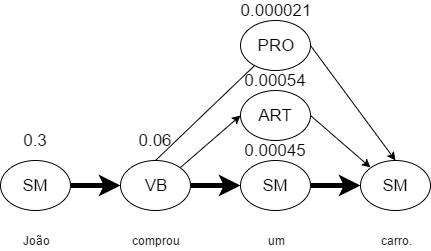
\includegraphics[height=180px]{imagens/markov2.png}
 \caption{Caminhos já decididos de classificação}
 \label{fig:markov2}
\end{figure}

Como visto, o método simbólico para resolver problemas de Processamento de
Linguagem Natural faz uso da criação de regras baseadas no conhecimento humano,
enquanto o método estatístico, decide através de cálculos probabilísticos
apoiados em estatísticas de um banco de dados para a resolução correta do
problema.


% Uma maneira de diferenciarmos os dois métodos é através do problema de
% ambiguidade. Por exemplo, nas frases:
% 
% ``João entrou no carro conversível de óculos novos.''. E ``João entrou no carro
% conversível de farol apagado.''.
% 
% Em ambas as frases, após a preposição ``de'' segue um substantivo masculino.
% Porém, cada uma das frases se refere a um substantivo diferente. A
% primeira se refere ao João, visto que não existe sentido em um carro ter óculos.
% Já a segunda se refere ao próprio carro, visto que não existe sentido em João
% ter faróis.
% 
% O método simbólico para resolver esse problema faz a criação de novas regras se
% baseadas no conhecimento humano para a solução de qual o significado da frase.
% Já o método estatístico, irá verificar qual a probabilidade de cada significado
% para cada frase através de análises similares decidindo através de metódos
% estatísticos qual o significado correto para cada frase
% \cite{jacksonmoulinier2007}.

\section{Métodos estatísticos e simbólicos aplicados na análise de sentimentos}
\label{cap:Classificadores}

%Para o \ac{NLP} e também para o campo de estatísticas, classificadores são
%algorítmos que identificam a qual categoria determinado item pertence. Essa
%classificação é feita a partir de dados já classificados corretamente, ou seja,
%um \textit{training set}.

\subsection{Naive Bayes}

O classificador Naive Bayes é um classificador baseado no teorema de Bayes com
independencia entre seus atributos.

O teorema de Bayes é representado da seguinte forma:

\[ P(c|d) = \frac{P(d|c) P(c)}{P(d)}  \]

Supondo que precisamos determinar se o carro que João comprou na frase ``João
comprou um Focus.'' é o modelo sedan ou hatch.
 
\begin{itemize}
  \item P(c$\vert$d) é a probabilidade de \textbf{d} pertencer a classe
  \textbf{c}. Ou seja, a probabilidade do carro Focus ser um sedan.
  \item P(d$\vert$c) é a probabilidade da classe \textbf{c} ser \textbf{d}. Ou
  seja, dentre todas as sedans, a probabilidade de um sedan ser
  um Focus.
  \item P(c) é a probabilidade da classe \textbf{c}. Ou seja, a frequência que
  sedans aparecem no nosso banco de dados.
  \item P(d) é a probabilidade de \textbf{d}. Ou seja, a frequência que Focus aparecem no nosso banco de dados.
\end{itemize}

Levando em consideração que temos o banco de dados representado pela tabela
abaixo:

\begin{table}[htb]
\centering
\label{123}
\begin{tabular}{|l|l|}
\hline
Carro  & Categoria \\ \hline
Focus  & Sedan     \\ \hline
Gol    & Hatch     \\ \hline
Focus  & Hatch     \\ \hline
Focus  & Sedan     \\ \hline
Focus  & Hatch     \\ \hline
Fox    & Hatch     \\ \hline
Fiesta & Hatch     \\ \hline
Cruze  & Sedan     \\ \hline
Focus  & Hatch     \\ \hline
\end{tabular} 
\caption{Tabela de Carro e Categoria.}
\end{table}

Probabilidade do Focus ser sedan:

\[ P(Sedan|Focus) = \frac{P(Focus|Sedan) P(Sedan)}{P(Focus)}  \]

\[ P(Sedan|Focus) = \frac{2/3 * 3/10}{5/10} = \frac{0,2}{0,5} = 0,4\]

Probabilidade do Focus ser um hatch:

\[ P(Hatch|Focus) = \frac{P(Focus|Hatch) P(Hatch)}{P(Focus)}  \]

\[ P(Hatch|Focus) = \frac{3/6 * 7/10}{5/10} = \frac{0,35}{0,5} = 0,7\]

No caso utilizado como exemplo, o Focus(Atributo ou \textit{Feature}) é um hatch
(Rótulo ou \textit{Label}).
Porém, caso tenhamos mais um atributo para utilizar na classificação o classificador Naive Bayes não
considera nenhuma dependência.
Como por exemplo a frase ``O carro era ano 2010 e tinha 2 portas'' com os
seguintes atributos:

\begin{table}[htb]
\centering
\begin{tabular}{|l|l|l|l|}
\hline
Carro  & Ano  & Portas & Categoria \\ \hline
Focus  & 2010 & 2      & Sedan     \\ \hline
Gol    & 2010 & 4      & Hatch     \\ \hline
Focus  & 2011 & 4      & Hatch     \\ \hline
Focus  & 2011 & 2      & Sedan     \\ \hline
Focus  & 2011 & 2      & Hatch     \\ \hline
Fox    & 2012 & 4      & Hatch     \\ \hline
Fiesta & 2012 & 2      & Hatch     \\ \hline
Cruze  & 2013 & 4      & Sedan     \\ \hline
Focus  & 2013 & 2      & Hatch     \\ \hline
\end{tabular}
\caption{Tabela de anos, carros, portas e categorias.}
\label{my-label}
\end{table}

O cálculo será feito da seguinte forma:

\[ P(d|c) = P(d_1|c) * P(d_2|c)* \ldots * P(d_n|c) \]

\[ P(Sedan|Focus) = P(Portas=2|Sedan) * P(Ano=2010|Sedan) \ldots * \]

\[ P(Sedan|Focus) = 2/3 * 1/3 \ldots * \]

Por assumir independência entre seus atributos, os valores obtidos nós cálculos
podem ser armazenados no banco de dados e reaproveitados. Por isso, sua
performance é considerada incrívelmente boa até mesmo para casos aonde temos forte dependência de
atributos \cite{domingos97naivebayes}.

%TODO EXEMPLO
\subsection{\textit{Maximum Entropy}}
O classificador \ac{MaxEnt} tem como
característica principal a preferência por modelos de dados uniformes sem efetuar nenhuma suposição injustificada.

Podemos utilizar um exemplo similar ao anterior para demonstrar a lógica do
classificador \ac{MaxEnt}. 
 
``João comprou um carro.''.

Supondo que temos que classificar o tipo de carro comprado em três categorias:

\begin{itemize}
  \item Hatch.
  \item Sedan.
  \item Cupê.
\end{itemize}

Podemos afirmar que:

\[ P(Hatch) + P (Sedan) + P(Cupe) = 1 \]

Como só temos essas três possibilidades de classificação no nosso
exemplo, o carro só pode ser classificado em uma dessas três possibilidades, ou
seja, a soma das três probabilidades deve ser 100\% ou 1 essa é a primeira
restrição ou \textit{constraint}. Abaixo duas tabelas que satisfazem essa
restrição:

\begin{table}[htb]
\centering
\begin{tabular}{|l|l|}
\hline
Tipo  & \%   \\ \hline
Sedan & 33\% \\ \hline
Hatch & 33\% \\ \hline
Cupê  & 33\% \\ \hline
 \end{tabular}
\caption{Tabela de Probabilidades A} 
\end{table}
\begin{table}[htb]
\centering
 \begin{tabular}{|l|l|}
\hline
Tipo  & \%   \\ \hline
Sedan & 50\% \\ \hline
Hatch & 50\% \\ \hline
Cupê  & 0\% \\ \hline
 \end{tabular}  
\caption{Tabela de Probabilidades B} 
\end{table}

Sem nenhum conhecimento prévio da distribuição desses carros, ou seja, a
quantidade de carros comprados por tipo, o classificador assume uma distribuição
uniforme das probabilidades, portanto, com maior entropia.

\begin{itemize}
  \item Hatch - 33\%.
  \item Sedan - 33\%.
  \item Cupê - 33\%.
\end{itemize}

Agora, supondo que a partir do nosso banco de dados conseguimos verificar que em
80\% dos casos o veículo comprado era um sedan ou hatch, temos uma nova
restrição:

\[ P(Hatch) + P (Sedan) = 0.8 \]

Podemos novamente ter n distribuições diferentes, porém a distribuição mais
uniforme que satisfaz as nossas duas restrições são:

\begin{itemize}
  \item Hatch - 40\%.
  \item Sedan - 40\%.
  \item Cupê - 30\%.
\end{itemize}

Esse é o princípio da Máxima Entropia utilizado nessa forma de classificação.
Primeiro é descoberta a frequência de cada atributo, depois é procurada a
distribuição que máximiza a entropia, ou seja, a mais uniforme.

%\subsection{Modelo Probabilístico}

%O seu modelo probabilístico para as probabilidades de observarmos o evento c
%quando d for verdadeiro:

%\[ P(c|d) := \frac{1}{Z(d)} exp (\Sigma_i\lambda_{i,c}F_{i,c}(d,c))\]





\subsection{\textit{VADER}}

O \ac{VADER} é um dicionário e classificador de sentimentos que se baseia em
regras, portanto, um método de classificação simbólico. Ele é especialmente
ajustado para funcionar em redes sociais aonde temos um contexto vago e pouca
quantidade de texto, nesse contexto, ele é extremamente eficaz, podendo se
comparar a classificação feita por humanos \cite{conf/icwsm/HuttoG14}.

Esse método faz uso de um dicionário que foi construído levando em consideração
gírias e emoticons utilizados em redes sociais. Neste dicionário as palavras
estão previamente associadas a uma polaridade de sentimento (positivo e
negativo) e intensidade em uma escala de -4 até +4, como por exemplo, a palavra
\textit{great} tem a intensidade de 3.1 e \textit{horrible} -2.5. Essa
associação foi construída utilizando o método de \textit{``wisdom of the
crowd''} aonde um grupo de pessoas atribuiu os valores para cada palavra ao
invés de somente uma pessoa especializada ou uma classificação automática
através de estatística.

Ele faz uso de cinco regras gerais:


\begin{itemize}
  \item Pontuação. O ponto de exclamação (!) aumenta a magnitude da
  intensidade sem modificar a orientação semântica. Como por exemplo,
  \textit{``This place is great!!!''} é mais intenso que \textit{``This place
  is great''}.
  \item Capitalização. Especificamente, uma palavra que é relevante para a
  análise de sentimentos, quando essa é escrita em letras maiúsculas, é
  aumentada a magnitude da intensidade do sentimento sem modificar a orientação
  semântica. Como por exemplo, na frase \textit{``This place is GREAT''}, temos
  a palavra \textit{``GREAT''} (Ótimo) que está relacionada com o sentimento
  positivo. Neste caso aonde ela está escrita em letras maiúsculas, ela é mais
  intensa que \textit{``This place is great''}.
  \item Advérbios intensificadores. Estes impactam a intensidade do sentimento
  aumentando ou diminuindo a intensidade do sentimento. Na frase \textit{``This
  place is extremelly good''} o advérbio \textit{extremelly} (extremamente)
  aumenta a intensidade do sentimento expresso pela frase (\textit{good} ou
  bom), enquanto na frase \textit{``This place is marginally good''}, a palavra
  \textit{``marginally'' ou marginalmente} acaba diminuindo a intensidade do
  sentimento expresso.
  \item A palavra \textit{``but''}. Essa palavra indica uma troca no sentimento
  da frase expressa aonde que o texto seguinte a ela expressa um sentimento mais
  dominante. Por exemplo, a frase \textit{``This place is great but today, the
  service was horrible''} convém um sentimento misto.
  \item Por fim, ao examinar as três palavras anteriores, o método consegue
  identificar 90\% dos casos aonde uma negação inverte a polaridade de um texto.
  Como por exemplo, na frase \textit{``This place isn't that great''}, a
  palavra \textit{great} demonstra um sentimento positivo, porém, ao analisar
  as três palavras anteriores \textit{``place isn't that''} encontramos uma
  negação, mudando o sentimento expresso da frase de positivo para negativo.
\end{itemize}


\chapter{Criação de Base de Dados}
\label{cap:banco}
Este capítulo tem como objetivo descrever a rede social Reddit.
Após, são apresentados os tópicos que foram selecionados para a análise de
sentimentos. Por fim, é apresentada a ferramenta desenvolvida para a extração
dos comentários destes tópicos e para a criação da base.
\section{Rede Social Reddit}
\label{cap:Reddit}

O \textit{website} Reddit foi criado por Alexis Ohanian e Steve Huffman e teve
seu início em 2005 como um agregador de conteúdo e, atualmente, é o vigésimo terceiro \textit{website} mais acessado na
internet e o sétimo mais acessado nos Estados Unidos da América \cite{alexa}.
Os usuários do Reddit podem enviar \textit{links} com conteúdos externos
ao Reddit ou ainda mensagens de texto. A partir desse conteúdo, os seus
usuários podem votar para cima (\textit{upvote}) ou para baixo \textit{downvote},
influenciando na posição do conteúdo no \textit{website}. Além de votar no conteúdo, seus usuários podem enviar comentários como
forma de expressar sua opinião (Figura \ref{fig:reddit}).

\newpage

\begin{figure}[!htbp]
\centering

\includegraphics[height=300px]{imagens/reddit.png}
\caption{\textit{Website Reddit}:  As flechas demarcadas permitem efetuarmos
\textit{upvotes} ou \textit{downvotes}.}
\label{fig:reddit}
\end{figure}

O conteúdo do Reddit é distribuído em \textit{subreddits} que funcionam como
comunidades. Os usuários podem se inscrever nesses
\textit{subreddits}, recebendo as atualizações na sua página inicial, sendo
que dentre esses \textit{subreddits}, destacam-se:


\begin{itemize}
  \item \textit{/r/AskReddit}: esse \textit{subreddit} é utilizado para fazer
  perguntas gerais para outros usuários do Reddit. Esse \textit{subreddit}
  possui aproximadamente 16.941.540 inscritos.
  \item \textit{/r/worldnews}: esse \textit{subreddit} possui as notícias de
  todo o mundo, contando com aproximadamente 16.570.600 inscritos.
  \item \textit{/r/IAmA}: IAmA é um estilização de 'I am a' ('Eu sou um'):
  a partir desse \textit{subreddit} os usuários podem fazer perguntas ao criador
  de um determinado tópico. Esse \textit{subreddit} possui aproximadamente
  16.990.160 inscritos.
\end{itemize}

% Dentre esses \textit{subreddits} podemos destacar alguns dos tópicos mais
% acessados no ano de 2016:
% 
% \begin{itemize}
%   \item \textit{/r/IAmA} - \textit{We're NASA scientists \& exoplanet experts.
%   Ask us anything about today's announcement of seven Earth-size planets
%   orbiting TRAPPIST-1!} - Tópico de perguntas e respostas com cientistas da
%   NASA após a descoberta dos planetas que orbitavam a estrela TRAPPIST-1.
%   \item \textit{/r/IAmA} - \textit{I’m Bill Gates, co-chair of the Bill \&
%   Melinda Gates Foundation. Ask Me Anything.} - Tópico de perguntas e respostas com Bill Gates.
%   \item \textit{/r/worldnews} - \textit{Fidel Castro is dead at 90.} - Link para
%   anúncio da morte de Fidel Castro.
%   \item \textit{/r/AskReddit} - \textit{[Serious]South Koreans of Reddit, how
%   did they teach you about the existence of North Korea in School when you were
%   young?serious replies only} - Tópico perguntando para os usuários sul coreanos
%   como que foi ensinado para eles sobre a existência da Coreia do Norte.
% \end{itemize}

% A identificação de padrões de sentimentos expressos por determinados grupos
% dessa comunidade, se faz útil visto que a partir dessa avaliação é possível construir
% ferramentas que apoiam decisões tanto de um ponto de vista político, como por
% exemplo, entender qual é a opinião sobre um determinado assunto de um conjunto
% de eleitores, tanto quanto um ponto de vista de negócios, para entender qual a
% opinião dos consumidores de um produto, ou de seu competidor, a respeito de um
% determinado assunto.

\section{Extração de Dados}
\label{cap:Extracao}

Para a extração comentários do \textit{website} Reddit e para a criação da base
foi desenvolvido um \textit{crawler} ou robô de navegação. Esse robô foi
implementado na linguagem Java e tem como objetivo a navegação automática no
conteúdo do \textit{website} Reddit, extraindo os dados e comentários referentes a um
determinado tópico. Após, os dados são armazenados em banco de dados MySQL
\cite{Widenius:2002:MRM:560480}.
Na Figura \ref{fig:crawler} tem-se a arquitetura do \textit{software}
desenvolvido. O código deste encontra-se no CD em anexo.

\begin{figure}[htbp]
\centering
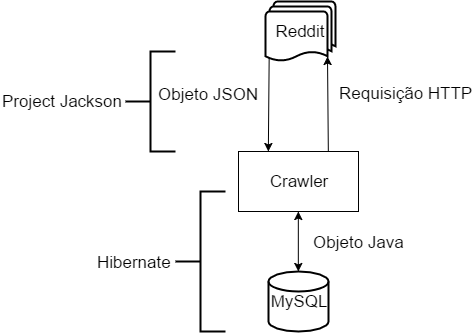
\includegraphics[height=225px]{imagens/arquitetura.png}
\caption{Arquitetura do \textit{Crawler}}
\label{fig:crawler}
\end{figure}

A partir de um \textit{link} para um tópico, o robô efetua uma busca e a
extração dos dados relacionados a esse tópico. Para tanto, foi utilizada a
\ac{API} do Reddit, onde, inicialmente envia-se uma requisição utilizando o
sufixo ``.json'' (Por exemplo:
\textit{\url{https://www.reddit.com/r/iama.json}}) e, a partir dessa requisição,
o \textit{website} retorna um objeto \ac{JSON}. Uma vez que o \ac{JSON}
retornado pelo \textit{website} possui 68 campos e que esses não se encontram
documentados, utilizou-se o \textit{website}
jsonschema2pojo\footnote{http://www.jsonschema2pojo.org/ - O \textit{website}
jsonschema2pojo tem como objetivo a conversão de um esquema \ac{JSON} em
\textit{Plain Old Java Objects}\ac{POJO}, permitindo o \textit{download} da classe para a utilização.} para converter o
JSON retornado em um \textit{Plain Old Java Objects} (\ac{POJO}).

Após, foi utilizado o \textit{framework} Hibernate
\cite{Iverson:2004:HJD:1044870} para a criação do banco de dados e para a
persistência dos dados. O Hibernate é um \textit{framework} de
mapeamento objeto-relacional que tem como objetivo representar tabelas do banco
de dados através de classes, ou seja, esse \textit{framework} tem como principal
característica a transformação das classes em Java para tabelas em um banco de dados relacional.
No caso deste trabalho, ele é responsável pela criação das tabelas \textit{RedditPost} e
\textit{RedditThread}, relacionadas, respectivamente, com os comentários e o
tópico em questão. 

\section{Tópicos Selecionados}

Para análise de sentimentos e para comparação dos resultados obtidos, foram
selecionados 15 tópicos, sendo que esses tópicos são os que
apresentam o maior número de comentários no último ano. Destaca-se que os 15
tópicos encontram-se distribuídos em diferentes assuntos, que são: cenário
político nacional, cenário político internacional e tópicos diversos:

No que diz respeito a tópicos relacionados com ao cenário político nacional, os
tópicos escolhidos foram:
\sloppy
\begin{itemize}
  \item
  \textit{Brazil Seeks To Copy U.S. Gun Culture ``to allow embattled
  citizens the right to defend themselves from
  criminals''}: esse tópico encontra-se disponível em 
  \url{https://www.reddit.com/r/worldnews/comments/36ny58/brazil_blogger_known_for_reporting_on_corruption/}
  e refere-se a intenção do Brasil em adotar a cultura de porte de armas dos
  Estados Unidos da América.
  \item
  \textit{Brazil descends into chaos as Olympics looms}: esse tópico encontra-se disponível em 
  \url{https://www.reddit.com/r/worldnews/comments/4bqcc3/brazil_descends_into_chaos_as_olympics_looms/}
  e refere-se ao caos ocorrido nas Olímpiadas de 2016 que foram realizadas no
  Brasil.
  \item
  \textit{Plane carrying Brazil Supreme Court judge crashes into sea}: esse tópico encontra-se disponível em
  \url{https://www.reddit.com/r/worldnews/comments/5oyz3b/plane_carrying_brazil_supreme_court_judge_crashes/}
  e refere-se a queda do avião no qual o ministro Teori Zavascki estava abordo.
  \item
  \textit{Brazil passes Internet governance Bill: Brazil has made history with
  the approval of a post-Snowden Bill which sets out principles, rights and
  guarantees for Internet users.}: esse tópico encontra-se disponível em
  \url{https://www.reddit.com/r/worldnews/comments/21f3as/brazil_passes_internet_governance_bill_brazil_has/}
  e refere-se a aprovação do Marco Civil da Internet.
  \item
  \textit{FIFA generated more than \$4 billion in sales from the 2014 World Cup,
  and is Giving Brazil \$100 Million After The Country Spent \$15 Billion On The
  World Cup}: esse tópico encontra-se disponível em
  \url{https://www.reddit.com/r/worldnews/comments/2t65ql/fifa_generated_more_than_4_billion_in_sales_from/}
  e refere-se a diferença entre o que foi gasto e o que foi arrecadado pelo
  Brasil na Copa do Mundo de 2014.
 
\end{itemize}

Já os tópicos escolhidos que se referem a política internacional são:
\begin{itemize}
  \item
  \textit{2.6 terabyte leak of Panamanian shell company data reveals "how a
  global industry led by major banks, legal firms, and asset management companies
  secretly manages the estates of politicians, Fifa officials, fraudsters and
  drug smugglers, celebrities and professional
  athletes."}.: esse tópico encontra-se disponível em
  \url{https://www.reddit.com/r/worldnews/comments/4d75i7/26_terabyte_leak_of_panamanian_shell_company_data/}
  e se refere ao vazamento dos documentos confidenciais de uma
  sociedade de advogados panamenha. Esses documentos apresentam informações
  detalhadas de empresas localizadas em paraísos fiscais.
  \item
  \textit{Fidel Castro is dead at
  90.}: esse tópico encontra-se disponível em
  \url{https://www.reddit.com/r/worldnews/comments/5exz2e/fidel_castro_is_dead_at_90/}
  e se refere a morte do presidente de Cuba, Fidel Castro.
  
  \item
  \textit{Donald Trump to strip all funding from State Dept team promoting
  women's rights around the world - Leaked plan comes as First Daughter Ivanka
  defends her father's record with women}: esse tópico encontra-se disponível em
  \url{https://www.reddit.com/r/worldnews/comments/67ivae/donald_trump_to_strip_all_funding_from_state_dept/}
  e refere-se a decisão do presidente dos Estados Unidos da América, Donald
  Trump, em remover fundos de promoção ao direito das mulheres.
  
  \item
  \textit{Manchester Arena 'explosions': Two loud bangs heard at MEN Arena}:
  esse tópico encontra-se disponível em
  \url{https://www.reddit.com/r/worldnews/comments/6cqdye/manchester_arena_explosions_two_loud_bangs_heard/}
  e refere-se ao atentado terrorista ocorrido na Manchester Arena (Inglaterra)
  em 23 de Maio de 2017.
  
  \item
  \textit{Sweden asks the U.S. to explain Trump comment on
  Sweden}: esse tópico encontra-se disponível em
  \url{https://www.reddit.com/r/worldnews/comments/5uzetf/sweden_asks_the_us_to_explain_trump_comment_on/}
  e se refere aos comentários feitos do presidente dos Estados Unidos da
  América, Donald Trump, sobre a Suécia.
  
  \item\textit{“Canada will welcome you,” Trudeau invites refugees as Trump bans
  them}: esse tópico encontra-se disponível em
  \url{https://www.reddit.com/r/worldnews/comments/5qqa51/canada_will_welcome_you_trudeau_invites_refugees/}
  e refere-se a declaração do primeiro ministro canadense sobre decisão de
  receber refugiados. Neste declaração, o primeiro ministro canadense afirma que
  os refugiados serão bem-vindos no Canadá.
\end{itemize}

Por fim, os tópicos selecionados que abordam assuntos diversos foram:
\begin{itemize}
  \item
  \textit{I’m Bill Gates, co-chair of the Bill \& Melinda Gates Foundation. Ask
  Me Anything.}: esse tópico encontra-se disponível em
  \url{https://www.reddit.com/r/IAmA/comments/5whpqs/im_bill_gates_cochair_of_the_bill_melinda_gates/}
  e apresenta as respostas de perguntas que foram feitas ao fundador
  da Microsoft, Bill Gates.
  \item
  \textit{Hey, it's Lars from Metallica. AMA}: esse tópico encontra-se disponível em
  \url{https://www.reddit.com/r/IAmA/comments/1wl9ic/hey_its_lars_from_metallica_ama/}.
  Esse tópico apresenta as respostas de perguntas que foram realizadas ao
  vocalista da banda de rock Metallica, James Hetfield.
  \item
  \textit{I'm the CEO of Renault and Nissan and we're making autonomous driving
  vehicles happen by 2020. Ask me anything!}: esse tópico encontra-se disponível em
  \url{https://www.reddit.com/r/IAmA/comments/2s7obx/im_the_ceo_of_renault_and_nissan_and_were_making/}
  e refere-se as respostas às perguntas realizadas ao diretor executivo da Renault e Nissan,
  Carlos Ghosn.
  
  \item
  \textit{I am Julian Assange founder of WikiLeaks -- Ask Me Anything}: esse
  tópico encontra-se disponível em
  \url{https://www.reddit.com/r/IAmA/comments/5n58sm/i_am_julian_assange_founder_of_wikileaks_ask_me/}
  e refere-se as respostas às perguntas realizadas ao Julian Assange, fundador do
  \textit{WikiLeaks}.
  
\end{itemize}


Destaca-se que para a criação da base de dados, somente foram extraídos
comentários em resposta ao tópico em questão, comentários em resposta a outros
comentários foram desconsiderados, uma vez que esses podem não estar diretamente
relacionados ao tópico em questão, tornando inválida ou prejudicando a análise de sentimento.


\chapter{Conclusão Parcial}
\label{cap:conclusao}
A \ac{NLP} tem como objetivo a análise de linguagem natural, seja
essa escrita ou falada. Dentre diversas tarefas que ela executa, tem-se a
análise de sentimentos, a qual recebeu destaque nos últimos anos devido ao fato das pessoas cada vez se comunicarem através de redes sociais,
gerando um grande volume de dados. A análise e quantificação da opinião expressa por esses dados, seja
por fins políticos, comerciais ou quaisquer outros, se torna díficil devido a
essa grande quantidade de dados.

Observou-se que os métodos mais utilizados para análise de sentimentos são o
Método de Naive Bayes (estatístico) e o Método de \ac{VADER} (simbólico). Dentre
estes, optou-se pela utilização do método de \ac{VADER}, uma vez que de acordo
com a literatura, esse apresenta um desempenho superior ao método de Naive
Bayes. De fato, esse mostrou-se superior na análise de sentimentos nas avaliações de
produtos da Amazon, editoriais do New York Times e mais importante, na análise
de \textit{Tweets} da rede social Twitter \cite{SentimentinSocialMedia}. A
justificativa para isso, se dá ao fato de métodos estatísticos necessitarem de um \textit{training set}
especializado para obter resultados similares ou superiores aos métodos
simbólicos. 

Além disso, optou-se pela utilização do método de \ac{VADER}, devido
ao fato deste não necessitar da criação de um \textit{training set} específico
para a análise de sentimentos. A necessidade da criação de um \textit{training
set} específico para cada tema inviabilizaria o desenvolvimento deste trabalho,
uma vez que neste serão analisados 15 tópicos com temas distintos. Para
implementação do método \ac{VADER} optou-se pela biblioteca \ac{NLTK}. A
utilização da biblioteca \ac{NLTK} permitirá a utilização futura de outros
métodos de \ac{NLP}, bem como um estudo da performance do Método de \ac{VADER} e esses outros métodos.
 
Por fim, se fez necessária a criação de uma base de dados para armazenar os
tópicos e os comentários disponibilizados pela rede social Reddit. Para isso,
foi desenvolvido um \textit{crawler} (robô) que é responsável por extrair os
comentários relacionados a um tópico na rede social Reddit e armazenar em um
banco de dados MySQL. Esse robô foi desenvolvido na linguagem Java e utiliza a
API da rede social Reddit para extrair as informações de um tópico. Após, ele
utiliza o \textit{framework} Hibernate para armazenar os dados extraídos na
base de dados MySQL.

Na segunda etapa deste trabalho, será utilizado o \textit{framework} \ac{NLTK}
para efetuar a análise de sentimento sobre a base de dados criada. Essa análise
tem como principal objetivo identificar padrões de sentimentos entre
usuários e comunidades da rede Reddit.

\section{Atividades e Cronograma}

Na Tabela \ref{tab:tcc1} tem-se o cronongrama das atividades realizadas durante
o TCC I. Como pode ser observado, todas as tarefas programadas foram
realizadas.
\begin{enumerate}
\item Estudo de algoritmos para o processamento de texto e também análise de
sentimentos.
\item Análise das ferramentas já existentes.
\item Análise da API do Reddit.
\item Construção de um software para extração dos dados da API.
\item Extração e criação da base de dados.
\item Redação da monografia TCC I.
\item Apresentação TCC I.
\end{enumerate}

\renewcommand{\arraystretch}{2}
\newcolumntype{Y}{>{\centering\arraybackslash}X}
\begin{table}[!htb]
\begin{tabularx}{0.9\textwidth}{Y|Y|Y|Y|Y|Y|Y|Y|Y|Y|Y|}
& \multicolumn{2}{|c|}{Mar} & \multicolumn{2}{|c|}{Abr} &
\multicolumn{2}{|c|}{Mai} & \multicolumn{2}{|c|}{Jun} &
\multicolumn{2}{|c|}{Jul}
\\
\midrule
1 & \cellcolor{black!80} & \cellcolor{black!80} & & & & & & & & \\
2 &  & \cellcolor{black!80} & \cellcolor{black!80} & & & & & & &\\
3 &  &  &  & \cellcolor{black!80} & & & & & &\\
4 &  &  &  &  & \cellcolor{black!80} & & & &  &\\
5 &  &  &  &  &  & \cellcolor{black!80} & \cellcolor{black!80} & & &\\
6 &  & \cellcolor{black!80}  & \cellcolor{black!80}  &  \cellcolor{black!80} & 
\cellcolor{black!80} & \cellcolor{black!80} & \cellcolor{black!80} & \cellcolor{black!80} &  &\\
7 &  &  &  &  &  & & & & \cellcolor{black!80} &\\
\end{tabularx}

\caption{Cronograma do TCC I.}
\label{tab:tcc1}
\end{table}

Já na Tabela \ref{tab:tcc2} tem-se as atividades a serem desenvolvidas no TCC
II:

\begin{enumerate}
\item Implementação do software de Processamento de Linguagem Natural para a
análise de sentimentos na base de dados criada.
\item Análise dos resultados obtidos.
\item Redação da monografia TCC II.
\item Apresentação do TCC II.
\end{enumerate}

\newcolumntype{Y}{>{\centering\arraybackslash}X}
\begin{table}[!htb]
\begin{tabularx}{0.9\textwidth}{Y|Y|Y|Y|Y|Y|Y|Y|Y|Y|Y|}
& \multicolumn{2}{|c|}{Ago} & \multicolumn{2}{|c|}{Set} &
\multicolumn{2}{|c|}{Out} & \multicolumn{2}{|c|}{Nov} &
\multicolumn{2}{|c|}{Dez}
\\
\midrule
1 & \cellcolor{black!80} & \cellcolor{black!80} & \cellcolor{black!80} &
\cellcolor{black!80} & & & & & & \\
2 &  & & & \cellcolor{black!80} & \cellcolor{black!80} & \cellcolor{black!80} &
& & &\\
3 &  & \cellcolor{black!80} & \cellcolor{black!80} & \cellcolor{black!80} &
\cellcolor{black!80} & \cellcolor{black!80} & \cellcolor{black!80}
& \cellcolor{black!80} & &\\
4 &  &  &  &  &  & & & & \cellcolor{black!80} &\\
\end{tabularx}

\caption{Cronograma do TCC II.}
\label{tab:tcc2}
\end{table}

% No Capítulo \ref{cap:Processamento} foram introduzidos dois tipos de métodos
% distintos para o \ac{NLP}, métodos simbólicos e
% métodos estatísticos, os quais foram estudados para a análise de sentimentos
% através do Capítulo \ref{cap:Classificadores}.
% 
% Através do Capítulo \ref{cap:Classificadores}, foram comparados um método
% simbólico e outro método estatístico a fim de se determinar qual apresenta melhor performance na análise de sentimentos
% aplicada em uma rede social, sendo que a literatura apontou que o método mais
% assertivo é o método \ac{VADER}, o qual está disponível através do
% \textit{framework} \ac{NLTK}.
% 
% Já no Capítulo \ref{cap:banco}, foi apresentada como funciona a rede social
% Reddit, os tópicos selecionados para a análise de sentimentos, e por fim foi
% apresentado a forma na qual esses tópicos serão extraídos para população da base
% de dados.
% 
% A partir das informações demonstradas através deste, deverá ser possível criar
% um \textit{software} que efetue a análise de dados utilizando o \ac{VADER},
% através do \textit{framework} \ac{NLTK}, aplicada nos tópicos demonstrados no
% Capítulo \ref{cap:banco}.




% ----------------------------------------------------------
% RESULTADOS
% ----------------------------------------------------------
%\part{Resultados}

%\chapter{Processamento de Linguagem Natural}
\label{cap:Processamento}

% Um computador, obviamente, está preparado para entender sua própria linguagem,
% como por exemplo, um compilador interpreta linhas de código fonte para gerar um
% programa executável seguindo exatamente o algoritmo utilizado. Por isso, temos o
% termo Natural no Processamento de Linguagem. 

O objetivo da área de Processamento de Linguagem Natural é analisar a linguagem natural, ou seja, a linguagem utilizada pelo seres humanos não
importando se essa é escrita ou falada \cite{manningschutze1999}.

O Processamento de Linguagem Natural é uma área antiga, sendo anterior a
invenção dos computadores modernos. De fato, sua primeira grande aplicação foi
um dicionário desenvolvido no Birkbeck College em Londres no ano de 1948. Por ser
uma área complexa, seus primeiros trabalhos foram notavelmente falhos o que
causou uma certa hostilidade por parte das agências formentadoras de pesquisas.

Os primeiros pesquisadores eram muitas vezes bilíngues, como por exemplo,
nativos alemães que imigraram para os Estados Unidos. Acreditava-se que pelo
fato desses terem conhecimento de ambas as linguas, Ingles e Alemão, eles teriam
capacidade de desenvolver programas de computadores que efetuariam a tradução das linguas
de modo satisfatório. Uma vez que esses encontraram muitas dificuldades,
ficou claro que o maior problema não era o conhecimento de ambas as
línguas e sim como expressar esse conhecimento na forma de um programa de
computador \cite{history}.

Para que um computador seja capaz de interpretar uma
língua, necessitamos antes entender como nós efetuamos essa
interpretação.
Por isso, uma parte considerável do Processamento de Linguagem Natural está apoiado na área de Linguística.

\section{Linguística}

O objetivo da Linguística é compreender como os humanos adquirem, produzem e
entendem as diversas línguas, ou seja, a forma com que conversamos, a nossa
escrita e outras mídias de comunicação \cite{manningschutze1999}.

Na linguagem tanto escrita, como na falada, existem regras que são utilizadas
para estruturar as expressões. Uma série de dificuldades no Processamento de
Linguagem Natural são ocasionadas pelo fato de que as pessoas constantemente
mudam essas regras para satisfazerem suas necessidades de comunicação
\cite{manningschutze1999}. Uma vez que as regras são constantemente modificadas pelo loucutor, se torna extremamente difícil a criação de um software ou hardware efetue a interpretação de uma língua. 


% \subsection{Sintaxe e Semântica}
% 
% No seu livro Estruturas Sintáticas, Noam Chomsky cita as seguintes frases
% ``Ideias verdes incolores dormem furiosamente'' e ``Incolores verde ideias dormem
% furiosamente''.
% 
% A primeira frase, do ponto de vista sintático é correta, porém, assim como a
% segunda frase, semânticamente não faz sentido.
% 
% O fato de que podemos modificar as regras da lingua de duas formas distintas é
% utilizado como evidência para a separação da sintaxe e semântica na língua.
% \cite{jacksonmoulinier2007}

\section{Métodos de Processamento de Linguagem Natural}

O \ac{NLP} tem como o objetivo a execução de diversas tarefas como categorização
de documentos, tradução e geração de textos a partir de um banco de dados de
computador, etc. Podemos destacar duas formas ou métodos para a execução dessas
tarefas, o método simbólico e o método estatístico, com origem o campo da linguística. 

Nos final dos anos 50 e 60, existiam excelentes métodos quantitativos
desenvolvidos durante a segunda guerra mundial para a solução de problemas
científicos \cite{shannon48}.
Porém, no ano de 1957, Chomsky publicou o seu trabalho ``Syntactic Structures''
e com isso, temos a primeira aparição da teoria de gramática gerativa, que
considera a gramática como um conjunto de regras. Essa abordagem através de um
conjunto de regras ao invés de um modelo matemático entra em conflito com os
trabalhos anteriores, criando duas comunidades no campo de Linguística. Como
reflexo das duas comunidades, a área de \ac{NLP} que crescia em paralelo a
linguística também foi dividida em duas, uma área que fazia uso de métodos que
utilizavam regras(simbólico) e uma outra área que fazia uso de métodos
quantitativos(estatísticos).


Essa seção tem como objetivo explicar os dois métodos principais de
abordagem e demonstrar as diferenças entre os dois métodos através de um exemplo
de desambiguação de categoria de palavras.


\subsection{Método Simbólico} 
O método simbólico ou racionalista está
baseado no campo da Linguística e faz o uso da manipulação dos símbolos,
significados e das regras de um texto. Um exemplo de método simbólico é o
método de Brill \cite{Brill:1992:SRP:974499.974526}. Por exemplo, no método de
Brill a frase ``João pintou a casa de branco'', será separada em palavras que
serão classificadas através de um dicionário pré-definido, como:

\begin{table}[htb]
\centering
\begin{tabular}{l|l|l|l|l|l|l}
Palavra         & João        & pintou & a      & casa        & de        
& branco
         \\
%Correta: & Substantivo & Verbo  & Artigo & Substantivo & Preposição &
% Substantivo \\
Classificação:   & 			   & Verbo  & Artigo & Substantivo & Preposição & Adjetivo
\end{tabular}
\label{my-label}
\end{table}

Observa-se que algumas palavras não foram
identificadas, como ``João'' ou classificadas de forma errada, como
``branco". Desta forma, o método utiliza-se de outras duas regras para uma
classificação inicial.
A primeira regra classifica todas as palavras desconhecidas que iniciam em
maiúsculo como substantivos, por exemplo, a palavra ``João''. Já a segunda regra, atribui para a palavra desconhecida a mesma classificação
de outras palavras que terminam com as mesmas três letras. Por exemplo, supondo
que a palavra ``pintou'' não fosse encontrada no dicionário, essa seria
associada a outras palavras terminadas com o sufixo ``tou''. Ou seja, essa seria
associada como verbo.

\begin{table}[htb]
\centering
\begin{tabular}{l|l|l|l|l|l|l}
Palavra         & João        & pintou & a      & casa        & de        
& branco
         \\
%Correta: & Substantivo & Verbo  & Artigo & Substantivo & Preposição &
% Substantivo \\
Classificação:   & \textbf{Substantivo} & Verbo  & Artigo & Substantivo &
Preposição & Adjetivo
\end{tabular}
\label{my-label}
\end{table}



Após essa classificação inicial, o método executa o seguinte conjunto de regras:

\begin{itemize}
   \item Se uma palavra tem a classificação \textbf{A} e está no contexto
  \textbf{C} então a sua classificação deverá ser mudada para \textbf{B}. Por
  exemplo, se uma palavra \textbf{A} (branco no exemplo) é um adjetivo e uma das
  duas palavras anteriores é uma preposição (``de'' no contexto \textbf{C}
  ), mude para sua classificação para substantivo (classificação \textbf{B}).
  
  \[\overbrace{\text{João}}^\text{Substantivo}
  \overbrace{\text{pintou}}^\text{Verbo}
  \overbrace{\text{a}}^\text{Artigo}
  \underbrace{
  \overbrace{\text{casa}}^\text{Substantivo}
  \overbrace{\text{de}}^\text{Preposição}}_\text{Contexto \textbf{C}}
  \underbrace{\overbrace{\text{branco}}^{\textcolor{red}{Adjetivo}}}_\text{Classificação
  \textbf{A}\textrightarrow\textbf{B}}
 \]
 
  \item Se uma palavra tem a classificação \textbf{A} e tem uma propriedade
  \textbf{P} então a sua classificação deverá ser alterada para \textbf{B}. Por
  exemplo, se uma palavra \textbf{A} (``Linda'') foi classificada como um
  adjetivo e é iniciada com uma letra maiúscula (propriedade \textbf{P}), sua
  classificação deverá ser alterada para substantivo (classificação \textbf{B}).
  
  \[\overbrace{\text{Comprei}}^\text{Verbo}
  \overbrace{\text{flores}}^\text{Substantivo}
  \overbrace{\text{para}}^\text{Preposição}
  \underbrace{\overbrace{\text{L}\text{inda}}^{\textcolor{red}{Adjetivo}}}_\text{Classificação
  \textbf{A}\textrightarrow\textbf{B}}
 \]
 
  \item Se uma palavra tem a classificação \textbf{A} e uma palavra com a
  propriedade \textbf{P} está na região \textbf{R}, sua classificação deverá
  ser \textbf{B}. Por exemplo, se uma das duas palavras anteriores (``João
  adora" na região \textbf{R}) iniciam com letra maiúscula (propriedade
  \textbf{P}), sua classificação deverá ser alterada para substantivo (classificação \textbf{B}).
  
   \[\underbrace{\overbrace{\text{João}}^\text{Substantivo}
  \overbrace{\text{adora}}^\text{Verbo}}_\text{Região \textbf{R}}
  \underbrace{\overbrace{\text{L}\text{inda}}^{\textcolor{red}{Adjetivo}}}_\text{Classificação
  \textbf{A}\textrightarrow\textbf{B}}
 \]
 
  
\end{itemize}

\subsection{Método Estatístico} 
O método estatístico ou empírico utiliza-se de grandes
quantidades de texto, procurando por padrões e
associações a modelos, sendo que esses podem ou não estarem relacionados com
regras sintáticas ou semânticas. Como exemplo, podemos citar a utilização de
Modelos de Markov pela algoritmo de Viterbi. Onde, a partir de um conjunto de
dados já classificados, ou seja, um \textit{training set} é verificada a
possibilidade de transição entre as classes gramaticais.
Por exemplo, se no nosso \textit{training set}, temos 10000 substantivos que em
7000 dos casos são seguidos por um verbo, temos:

\[ P(VB|SM) = \frac{C(SM,VB)}{C(SM)} = \frac{7000}{10000} = 0.7 \]

Onde \textbf{VB} são verbos e \textbf{SM} substantivos. Como pode ser observado
na equação, a probabilidade de um substantivo ser seguido de um verbo
(\textbf{(VB$\vert$SM)}) é igual a ocorrência de substantivos seguidos de verbos (\textbf{C(SM,VB)})
dividida pela quantidade total de substantivos em nosso \textit{training set}.

Após, é calculada a probabilidade de cada palavra ser associada com uma classe.
Supondo que dos 10000 substantivos, 150 são a palavra ``um'' classificada
dentre artigo, substantivo e pronome, como substantivo:

\[ P(um|SM) = \frac{C(SM,um)}{C(SM)} = \frac{150}{10000} = 0.015 \]

Aonde que \textbf{um} é a palavra que está sendo classificada e \textbf{SM}
são os substantivos existentes no nosso \textit{training set}. Portanto a
probabilidade de um substantivo ser associada a palavra ``um''
(\textbf{P(um$\vert$SM)}) é igual a quantidade da palavra ``um''
classificada como substantivo (\textbf{C(SM,um)}) dividida pela quantidade de
substantivos em nosso \textit{training set}.
Como exemplo, vamos supor os seguintes dados compilados através dos dois métodos
citados anteriormente, aonde a primeira tabela representa a probabilidade de
transição e a segunda tabela representa a probabilidade de associação:

\begin{table}[htb]
\centering
\begin{tabular}{|l|l|l|l|l|}
\hline
            & Substantivo & Verbo & Artigo & Pronome \\ \hline
Início      & 0.30        & 0.25  & 0.35   & 0.4     \\ \hline
Substantivo & 0.4         & 0.2   & 0.015  & 0.85    \\ \hline
Verbo       & 0.5         & 0.2   & 0.3    & 0.07    \\ \hline
Artigo      & 0.1         & 0.001 & 0.030  & 0.005   \\ \hline
Pronome     & 0.7         & 0.005 & 0.005  & 0.8     \\ \hline
\end{tabular}
\caption{Tabela de Probabilidade de Transição}
\label{tabela:transicao}
\end{table} 

\begin{table}[htb]
\centering
\begin{tabular}{|l|l|l|l|l|}
\hline
            & João & comprou & um    & carro \\ \hline
Substantivo & 1    &         & 0.015 & 1     \\ \hline
Verbo       &      & 1       &       &       \\ \hline
Artigo      &      &         & 0.030 &       \\ \hline
Pronome     &      &         & 0.005 &       \\ \hline
\end{tabular}
\caption{Tabela de Probabilidades de Associação}
\label{tabela:associacao}
\end{table}


Portanto, para a classificação da frase anterior, as palavras João, Comprou
e Carro, só podem ser classificadas como substantivo (SM), verbo (VB) e
substantivo (SM) respectivamente. Porém, a palavra ``um" pode ser classificada
em substantivo (SM), artigo (ART) e pronome (PRO). A seguinte imagem representa
as possibilidades de caminho que o classificador pode percorrer neste exemplo:

\begin{figure}[htbp]
 \centering
 \includegraphics[height=180px]{imagens/markov.png}
 \caption{Caminhos possíveis de classificação}
 \label{fig:markov}
\end{figure}

\newpage
Para a identificação da classe da palavra ``um'' é realizada a seguinte equação
seguindo o caminho representado pela figura anterior, começando pela palavra
João:

\[ v_t(j) = v_{t-1} a_{ij} b_j(o_t) \]

Aonde que $v_t$ é a probabilidade do caminho atual, $v_{t-1}$ é a
probabilidade do caminho anterior, $a_{ij}$ é a probabilidade de transição e $b_j(o_t)$ é a
probabilidade de associação.

Portanto a palavra ``João'', $v_{t-1}$ é representada pelo valor 1, visto
que essa é a primeira palavra e não existe probabilidade de caminho
anterior, $a_{ij}$ é a probabilidade de transição entre ``Início'' e um
substantivo, disponível na tabela \ref{tabela:transicao} e $b_j(o_t)$ é
a probabilidade de associação da palavra João com substantivo, disponível na
tabela \ref{tabela:associacao}:

\[ v_t(j) = 1 * 0.3 * 1 = 0.3 \]

Para ``comprou'', além dos valores retirados das tabelas \ref{tabela:transicao}
e \ref{tabela:associacao}, $v_{t-1}$ é representado pelo cálculo anterior do
caminho anterior, ou seja, 0.3:

\[ v_t(j) = 0.3 * 0.2 * 1 = 0.06 \] 

Ao efetuar o cálculo de todos os caminhos, para determinar qual a classificação
correta de uma palavra, é escolhido o caminho que tem maior probabilidade, no
caso apresentado, a palavra ``um'' é classificada como artigo.

\begin{figure}[htbp]
 \centering
 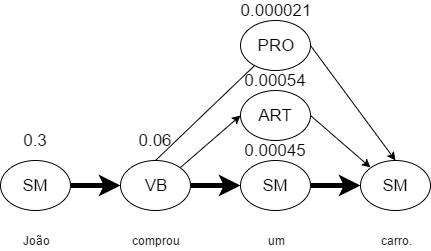
\includegraphics[height=180px]{imagens/markov2.png}
 \caption{Caminhos já decididos de classificação}
 \label{fig:markov2}
\end{figure}

Como visto, o método simbólico para resolver problemas de Processamento de
Linguagem Natural faz uso da criação de regras baseadas no conhecimento humano,
enquanto o método estatístico, decide através de cálculos probabilísticos
apoiados em estatísticas de um banco de dados para a resolução correta do
problema.


% Uma maneira de diferenciarmos os dois métodos é através do problema de
% ambiguidade. Por exemplo, nas frases:
% 
% ``João entrou no carro conversível de óculos novos.''. E ``João entrou no carro
% conversível de farol apagado.''.
% 
% Em ambas as frases, após a preposição ``de'' segue um substantivo masculino.
% Porém, cada uma das frases se refere a um substantivo diferente. A
% primeira se refere ao João, visto que não existe sentido em um carro ter óculos.
% Já a segunda se refere ao próprio carro, visto que não existe sentido em João
% ter faróis.
% 
% O método simbólico para resolver esse problema faz a criação de novas regras se
% baseadas no conhecimento humano para a solução de qual o significado da frase.
% Já o método estatístico, irá verificar qual a probabilidade de cada significado
% para cada frase através de análises similares decidindo através de metódos
% estatísticos qual o significado correto para cada frase
% \cite{jacksonmoulinier2007}.

\section{Métodos estatísticos e simbólicos aplicados na análise de sentimentos}
\label{cap:Classificadores}

%Para o \ac{NLP} e também para o campo de estatísticas, classificadores são
%algorítmos que identificam a qual categoria determinado item pertence. Essa
%classificação é feita a partir de dados já classificados corretamente, ou seja,
%um \textit{training set}.

\subsection{Naive Bayes}

O classificador Naive Bayes é um classificador baseado no teorema de Bayes com
independencia entre seus atributos.

O teorema de Bayes é representado da seguinte forma:

\[ P(c|d) = \frac{P(d|c) P(c)}{P(d)}  \]

Supondo que precisamos determinar se o carro que João comprou na frase ``João
comprou um Focus.'' é o modelo sedan ou hatch.
 
\begin{itemize}
  \item P(c$\vert$d) é a probabilidade de \textbf{d} pertencer a classe
  \textbf{c}. Ou seja, a probabilidade do carro Focus ser um sedan.
  \item P(d$\vert$c) é a probabilidade da classe \textbf{c} ser \textbf{d}. Ou
  seja, dentre todas as sedans, a probabilidade de um sedan ser
  um Focus.
  \item P(c) é a probabilidade da classe \textbf{c}. Ou seja, a frequência que
  sedans aparecem no nosso banco de dados.
  \item P(d) é a probabilidade de \textbf{d}. Ou seja, a frequência que Focus aparecem no nosso banco de dados.
\end{itemize}

Levando em consideração que temos o banco de dados representado pela tabela
abaixo:

\begin{table}[htb]
\centering
\label{123}
\begin{tabular}{|l|l|}
\hline
Carro  & Categoria \\ \hline
Focus  & Sedan     \\ \hline
Gol    & Hatch     \\ \hline
Focus  & Hatch     \\ \hline
Focus  & Sedan     \\ \hline
Focus  & Hatch     \\ \hline
Fox    & Hatch     \\ \hline
Fiesta & Hatch     \\ \hline
Cruze  & Sedan     \\ \hline
Focus  & Hatch     \\ \hline
\end{tabular} 
\caption{Tabela de Carro e Categoria.}
\end{table}

Probabilidade do Focus ser sedan:

\[ P(Sedan|Focus) = \frac{P(Focus|Sedan) P(Sedan)}{P(Focus)}  \]

\[ P(Sedan|Focus) = \frac{2/3 * 3/10}{5/10} = \frac{0,2}{0,5} = 0,4\]

Probabilidade do Focus ser um hatch:

\[ P(Hatch|Focus) = \frac{P(Focus|Hatch) P(Hatch)}{P(Focus)}  \]

\[ P(Hatch|Focus) = \frac{3/6 * 7/10}{5/10} = \frac{0,35}{0,5} = 0,7\]

No caso utilizado como exemplo, o Focus(Atributo ou \textit{Feature}) é um hatch
(Rótulo ou \textit{Label}).
Porém, caso tenhamos mais um atributo para utilizar na classificação o classificador Naive Bayes não
considera nenhuma dependência.
Como por exemplo a frase ``O carro era ano 2010 e tinha 2 portas'' com os
seguintes atributos:

\begin{table}[htb]
\centering
\begin{tabular}{|l|l|l|l|}
\hline
Carro  & Ano  & Portas & Categoria \\ \hline
Focus  & 2010 & 2      & Sedan     \\ \hline
Gol    & 2010 & 4      & Hatch     \\ \hline
Focus  & 2011 & 4      & Hatch     \\ \hline
Focus  & 2011 & 2      & Sedan     \\ \hline
Focus  & 2011 & 2      & Hatch     \\ \hline
Fox    & 2012 & 4      & Hatch     \\ \hline
Fiesta & 2012 & 2      & Hatch     \\ \hline
Cruze  & 2013 & 4      & Sedan     \\ \hline
Focus  & 2013 & 2      & Hatch     \\ \hline
\end{tabular}
\caption{Tabela de anos, carros, portas e categorias.}
\label{my-label}
\end{table}

O cálculo será feito da seguinte forma:

\[ P(d|c) = P(d_1|c) * P(d_2|c)* \ldots * P(d_n|c) \]

\[ P(Sedan|Focus) = P(Portas=2|Sedan) * P(Ano=2010|Sedan) \ldots * \]

\[ P(Sedan|Focus) = 2/3 * 1/3 \ldots * \]

Por assumir independência entre seus atributos, os valores obtidos nós cálculos
podem ser armazenados no banco de dados e reaproveitados. Por isso, sua
performance é considerada incrívelmente boa até mesmo para casos aonde temos forte dependência de
atributos \cite{domingos97naivebayes}.

%TODO EXEMPLO
\subsection{\textit{Maximum Entropy}}
O classificador \ac{MaxEnt} tem como
característica principal a preferência por modelos de dados uniformes sem efetuar nenhuma suposição injustificada.

Podemos utilizar um exemplo similar ao anterior para demonstrar a lógica do
classificador \ac{MaxEnt}. 
 
``João comprou um carro.''.

Supondo que temos que classificar o tipo de carro comprado em três categorias:

\begin{itemize}
  \item Hatch.
  \item Sedan.
  \item Cupê.
\end{itemize}

Podemos afirmar que:

\[ P(Hatch) + P (Sedan) + P(Cupe) = 1 \]

Como só temos essas três possibilidades de classificação no nosso
exemplo, o carro só pode ser classificado em uma dessas três possibilidades, ou
seja, a soma das três probabilidades deve ser 100\% ou 1 essa é a primeira
restrição ou \textit{constraint}. Abaixo duas tabelas que satisfazem essa
restrição:

\begin{table}[htb]
\centering
\begin{tabular}{|l|l|}
\hline
Tipo  & \%   \\ \hline
Sedan & 33\% \\ \hline
Hatch & 33\% \\ \hline
Cupê  & 33\% \\ \hline
 \end{tabular}
\caption{Tabela de Probabilidades A} 
\end{table}
\begin{table}[htb]
\centering
 \begin{tabular}{|l|l|}
\hline
Tipo  & \%   \\ \hline
Sedan & 50\% \\ \hline
Hatch & 50\% \\ \hline
Cupê  & 0\% \\ \hline
 \end{tabular}  
\caption{Tabela de Probabilidades B} 
\end{table}

Sem nenhum conhecimento prévio da distribuição desses carros, ou seja, a
quantidade de carros comprados por tipo, o classificador assume uma distribuição
uniforme das probabilidades, portanto, com maior entropia.

\begin{itemize}
  \item Hatch - 33\%.
  \item Sedan - 33\%.
  \item Cupê - 33\%.
\end{itemize}

Agora, supondo que a partir do nosso banco de dados conseguimos verificar que em
80\% dos casos o veículo comprado era um sedan ou hatch, temos uma nova
restrição:

\[ P(Hatch) + P (Sedan) = 0.8 \]

Podemos novamente ter n distribuições diferentes, porém a distribuição mais
uniforme que satisfaz as nossas duas restrições são:

\begin{itemize}
  \item Hatch - 40\%.
  \item Sedan - 40\%.
  \item Cupê - 30\%.
\end{itemize}

Esse é o princípio da Máxima Entropia utilizado nessa forma de classificação.
Primeiro é descoberta a frequência de cada atributo, depois é procurada a
distribuição que máximiza a entropia, ou seja, a mais uniforme.

%\subsection{Modelo Probabilístico}

%O seu modelo probabilístico para as probabilidades de observarmos o evento c
%quando d for verdadeiro:

%\[ P(c|d) := \frac{1}{Z(d)} exp (\Sigma_i\lambda_{i,c}F_{i,c}(d,c))\]





\subsection{\textit{VADER}}

O \ac{VADER} é um dicionário e classificador de sentimentos que se baseia em
regras, portanto, um método de classificação simbólico. Ele é especialmente
ajustado para funcionar em redes sociais aonde temos um contexto vago e pouca
quantidade de texto, nesse contexto, ele é extremamente eficaz, podendo se
comparar a classificação feita por humanos \cite{conf/icwsm/HuttoG14}.

Esse método faz uso de um dicionário que foi construído levando em consideração
gírias e emoticons utilizados em redes sociais. Neste dicionário as palavras
estão previamente associadas a uma polaridade de sentimento (positivo e
negativo) e intensidade em uma escala de -4 até +4, como por exemplo, a palavra
\textit{great} tem a intensidade de 3.1 e \textit{horrible} -2.5. Essa
associação foi construída utilizando o método de \textit{``wisdom of the
crowd''} aonde um grupo de pessoas atribuiu os valores para cada palavra ao
invés de somente uma pessoa especializada ou uma classificação automática
através de estatística.

Ele faz uso de cinco regras gerais:


\begin{itemize}
  \item Pontuação. O ponto de exclamação (!) aumenta a magnitude da
  intensidade sem modificar a orientação semântica. Como por exemplo,
  \textit{``This place is great!!!''} é mais intenso que \textit{``This place
  is great''}.
  \item Capitalização. Especificamente, uma palavra que é relevante para a
  análise de sentimentos, quando essa é escrita em letras maiúsculas, é
  aumentada a magnitude da intensidade do sentimento sem modificar a orientação
  semântica. Como por exemplo, na frase \textit{``This place is GREAT''}, temos
  a palavra \textit{``GREAT''} (Ótimo) que está relacionada com o sentimento
  positivo. Neste caso aonde ela está escrita em letras maiúsculas, ela é mais
  intensa que \textit{``This place is great''}.
  \item Advérbios intensificadores. Estes impactam a intensidade do sentimento
  aumentando ou diminuindo a intensidade do sentimento. Na frase \textit{``This
  place is extremelly good''} o advérbio \textit{extremelly} (extremamente)
  aumenta a intensidade do sentimento expresso pela frase (\textit{good} ou
  bom), enquanto na frase \textit{``This place is marginally good''}, a palavra
  \textit{``marginally'' ou marginalmente} acaba diminuindo a intensidade do
  sentimento expresso.
  \item A palavra \textit{``but''}. Essa palavra indica uma troca no sentimento
  da frase expressa aonde que o texto seguinte a ela expressa um sentimento mais
  dominante. Por exemplo, a frase \textit{``This place is great but today, the
  service was horrible''} convém um sentimento misto.
  \item Por fim, ao examinar as três palavras anteriores, o método consegue
  identificar 90\% dos casos aonde uma negação inverte a polaridade de um texto.
  Como por exemplo, na frase \textit{``This place isn't that great''}, a
  palavra \textit{great} demonstra um sentimento positivo, porém, ao analisar
  as três palavras anteriores \textit{``place isn't that''} encontramos uma
  negação, mudando o sentimento expresso da frase de positivo para negativo.
\end{itemize}



% ----------------------------------------------------------
% Finaliza a parte no bookmark do PDF
% para que se inicie o bookmark na raiz
% e adiciona espaço de parte no Sumário
% ----------------------------------------------------------
%\phantompart

% ---
% Conclusão (outro exemplo de capítulo sem numeração e presente no sumário)
% ---
%\chapter*[Conclusão]{Conclusão}
%\addcontentsline{toc}{chapter}{Conclusão}
% ---


% ----------------------------------------------------------
% ELEMENTOS PÓS-TEXTUAIS
% ----------------------------------------------------------
\postextual
% ----------------------------------------------------------

% ----------------------------------------------------------
% Referências bibliográficas
% ----------------------------------------------------------
\bibliographystyle{abntex2-alf}
\bibliography{tcc}

% ----------------------------------------------------------
% Glossário
% ----------------------------------------------------------
%
% Consulte o manual da classe abntex2 para orientações sobre o glossário.
%
%\glossary

% ----------------------------------------------------------
% Apêndices
% ----------------------------------------------------------

% ---
% Inicia os apêndices
% ---
%\include{diversos/apendices}
% ---


% ----------------------------------------------------------
% Anexos
% ----------------------------------------------------------
%\include{diversos/anexos}

%---------------------------------------------------------------------
% INDICE REMISSIVO
%---------------------------------------------------------------------
%\phantompart
%\printindex
%---------------------------------------------------------------------

\end{document}
